% !TEX root = ../thesis.tex
\chapter{Movish system}
\label{chapter:movish_system}

\section{Introduction}
\label{sec:movish_system_introduction}

In this chapter we will analyze the Movish automatic recommendation system deeply in all its aspects and we will show how the various challenges of implementing a real world recommendation system can be solved by either architecture or smart intuitions.

The reader will be guided on a tour that will include the project architecture, the project directory structure, the mechanism for automatic discovery of algorithms, the item crawler and the mechanism to hide the generated traffic in order to do not cause traffic throttling by the contacted servers.

\section{Architecture}
\label{sec:architecture}

Differently from ContentWise, a monolitic application, and from Milo, a fully separated application, Movish sits in the middle: it is a modular application. The \ac{GUI} and the recommendation engine are in the same application but are two different modules that cooperate in order to limit the point of failures (that were too spread on Milo) and allow flexibility.

\begin{figure}
  \centering
  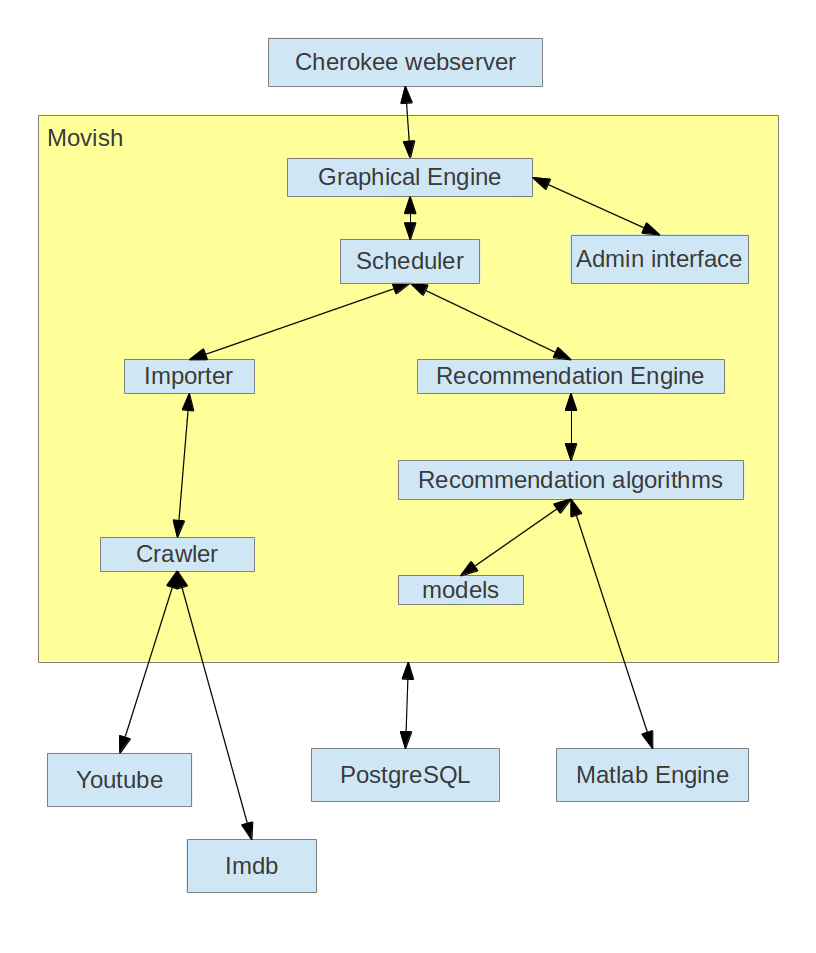
\includegraphics[width=\textwidth]{figures/movish_architecture.png}
  \caption{Movish architecture}
  \label{fig:movish_architecture}
\end{figure}

The architecture of the system can be see on Figure \ref{fig:movish_architecture}.
The system is exposed to internet(working) thanks to a cherokee web server \cite{cherokee}. Cherokee is an innovative, feature rich, and yet easy to configure open source web server. Its goal is to be as fast as it can and serve as many user as the hardware can hold. It is also C10K problem \cite{c10k-problem} aware. The C10k problem is the problem of serving 10.000 concurrent connections with commodity hardware, it has been well studied and only few webservers have been designed to address this problem.

Cherokee has been chosen for this project because it resulted to be both flexible and fast. Other webserver have been evaluated like nginx and apache. The first one was very good in benchmarks but lacked in flexibility, the latter was very modular but less likely to scale as soon users grow or the system is under heavy load, which is the case while a recommendation is performed while a model is being created.

Movish core modules are the graphical engine and the scheduler which have their basis on the web2py \cite{web2py} framework. The graphical engine speaks to the webserver thank to an application handler called uWSGI \cite{uwsgi}. uWSGI is an extremely advanced, sysadmin-friendly, highly-modular application container server written in POSIX-compatible C. It is the glue that connect the webserer with the application. As for the webserver, uWSGI has been chosen for its benchmarks and its lightweight.

The application relays in two other software and two services to work:
\begin{itemize}
\item A matlab \cite{matlab} engine executable installed in the local appliance. This is needed to perform the various operations with the algorithms that are written in matlab.
\item A PostgreSQL \cite{postgresql} database either remote or local. The database is the primary source of information for various parts of the executable. It is mainly used by the graphical engine, to get information to display about movies and users, and from the scheduler to coordinate all the workers for all the tasks. The importer also uses the database in order to store the crawled data.
\item Imdb.com. An internet access is required to access imdb.com as a primary source for new movies and useful information like release dates, plot, reviews and thus ratings. In fact the whole basic dataset has been built from the ground up crawling information about popular e latest movies of Imdb.com
\item Youtube.com or youtu.be. As for imdb.com, an internet connection is required to reach this service. The youtube source is used to search and retrieve the correct trailer to bind to the movie at database level.
\end{itemize}

Movish is a complex application that can be divided in different areas:
\begin{itemize}
\item Graphical engine. This is the core of the \ac{MVC} structure. It is responsible of answering the requests from the user, elaborate data and display the output.
\item Admin interface. This is the administrator specific part that is used to administrate the whole application from model creation, data retrieval, configuration of the algorithms, importing of new movies, administrate the scheduler, create new surveys and retrieve system information and status.
\item Scheduler. This component has the main task of taking computational intensive operations and execute in a separate process, then populate the database with the result of the computation. Since most of the operations with matrices are very computational intensive this module is heavy used by all the parts of the application.
\item Importer. It is the component that calls the crawler and manages the information from the crawler in an ordered way for storing into the database.
\item Crawler. It is responsible for getting all the information it can from imdb.com and youtube.com based on a movie or a set of movies. It is also able to parse imdb user pages and their ratings. It is most used by the task that update a movie given a movie id.
\item Recommendation engine. This component takes care of managing the communication with the Matlab engine. Since most of the operations of this module are very computationally expensive, this module is very used by the scheduler.
\item Recommendation algorithms. Those are all the matlab algorithms placed in a specific folder of the project. There is a logic to detect all the algorithms in a subtree of directories.
\item Models. As described in section \ref{sec:Stack}, models need to be created to perform the recommendation. This component manages all the created models for each algorithm in the system.
\end{itemize}

\subsection{Graphical Engine}
\label{sec:graphical-engine}

The graphical engine takes advantage of the web2py \cite{web2py} framework. A request is taken by the controller, the correct function to be executed is selected thank to the automatic route that find the function based on the project directory structure. When the function is executed it retrieves data from the database and populates a html template that is thus sent back to the user browser.

The graphical engine has two modes: normal and admin mode. Only users that have been promoted to admin are allowed to see the admin mode. To switch from one mode another the user can click on the admin link right after the login. The link is visible in figure \ref{fig:modes}. 

\begin{figure}
  \centering
  
\includegraphics[width=\textwidth]{figures/admin_mode.png}
  \caption{Admin and normal mode}
  \label{fig:modes}
\end{figure}

In Figure \ref{fig:movish_homepage} the reader can see the movish.co homepage as seen by a normal logged in or not logged in user which resembles the normal mode.
The layout has been inspired by pinterest, a popular social network for images but it has some peculiarities that makes it different for different reasons. The main difference from pinterest is the presence of a slider placed exactly at line of sight of the user, in the right position after the header and the Movish logo. The slider displays two sets of data: if the user is not logged in, it displays the most popular movies, if the user is logged in, it displays a recommendation generated by a random algorithm or a administrator defined one. So the user is forced, at first, to have a look at the recommendation or at the most popular movies. Scrolling down the page the user can start browsing the catalog via a search field or by seeing the different pages of the newly added items. In fact, by default, the list of movies that appears in the homepage represent the recently updated or inserted movies.

The fact that having a picture and a small text is the best way to display items \cite{using-collaborative-filtering} has been kept displaying the movie cover, the title, the release year and the genres. This allows to fit a movie in a small portion of the page but display enough amount of information to the user. 

\begin{figure}
  \centering
  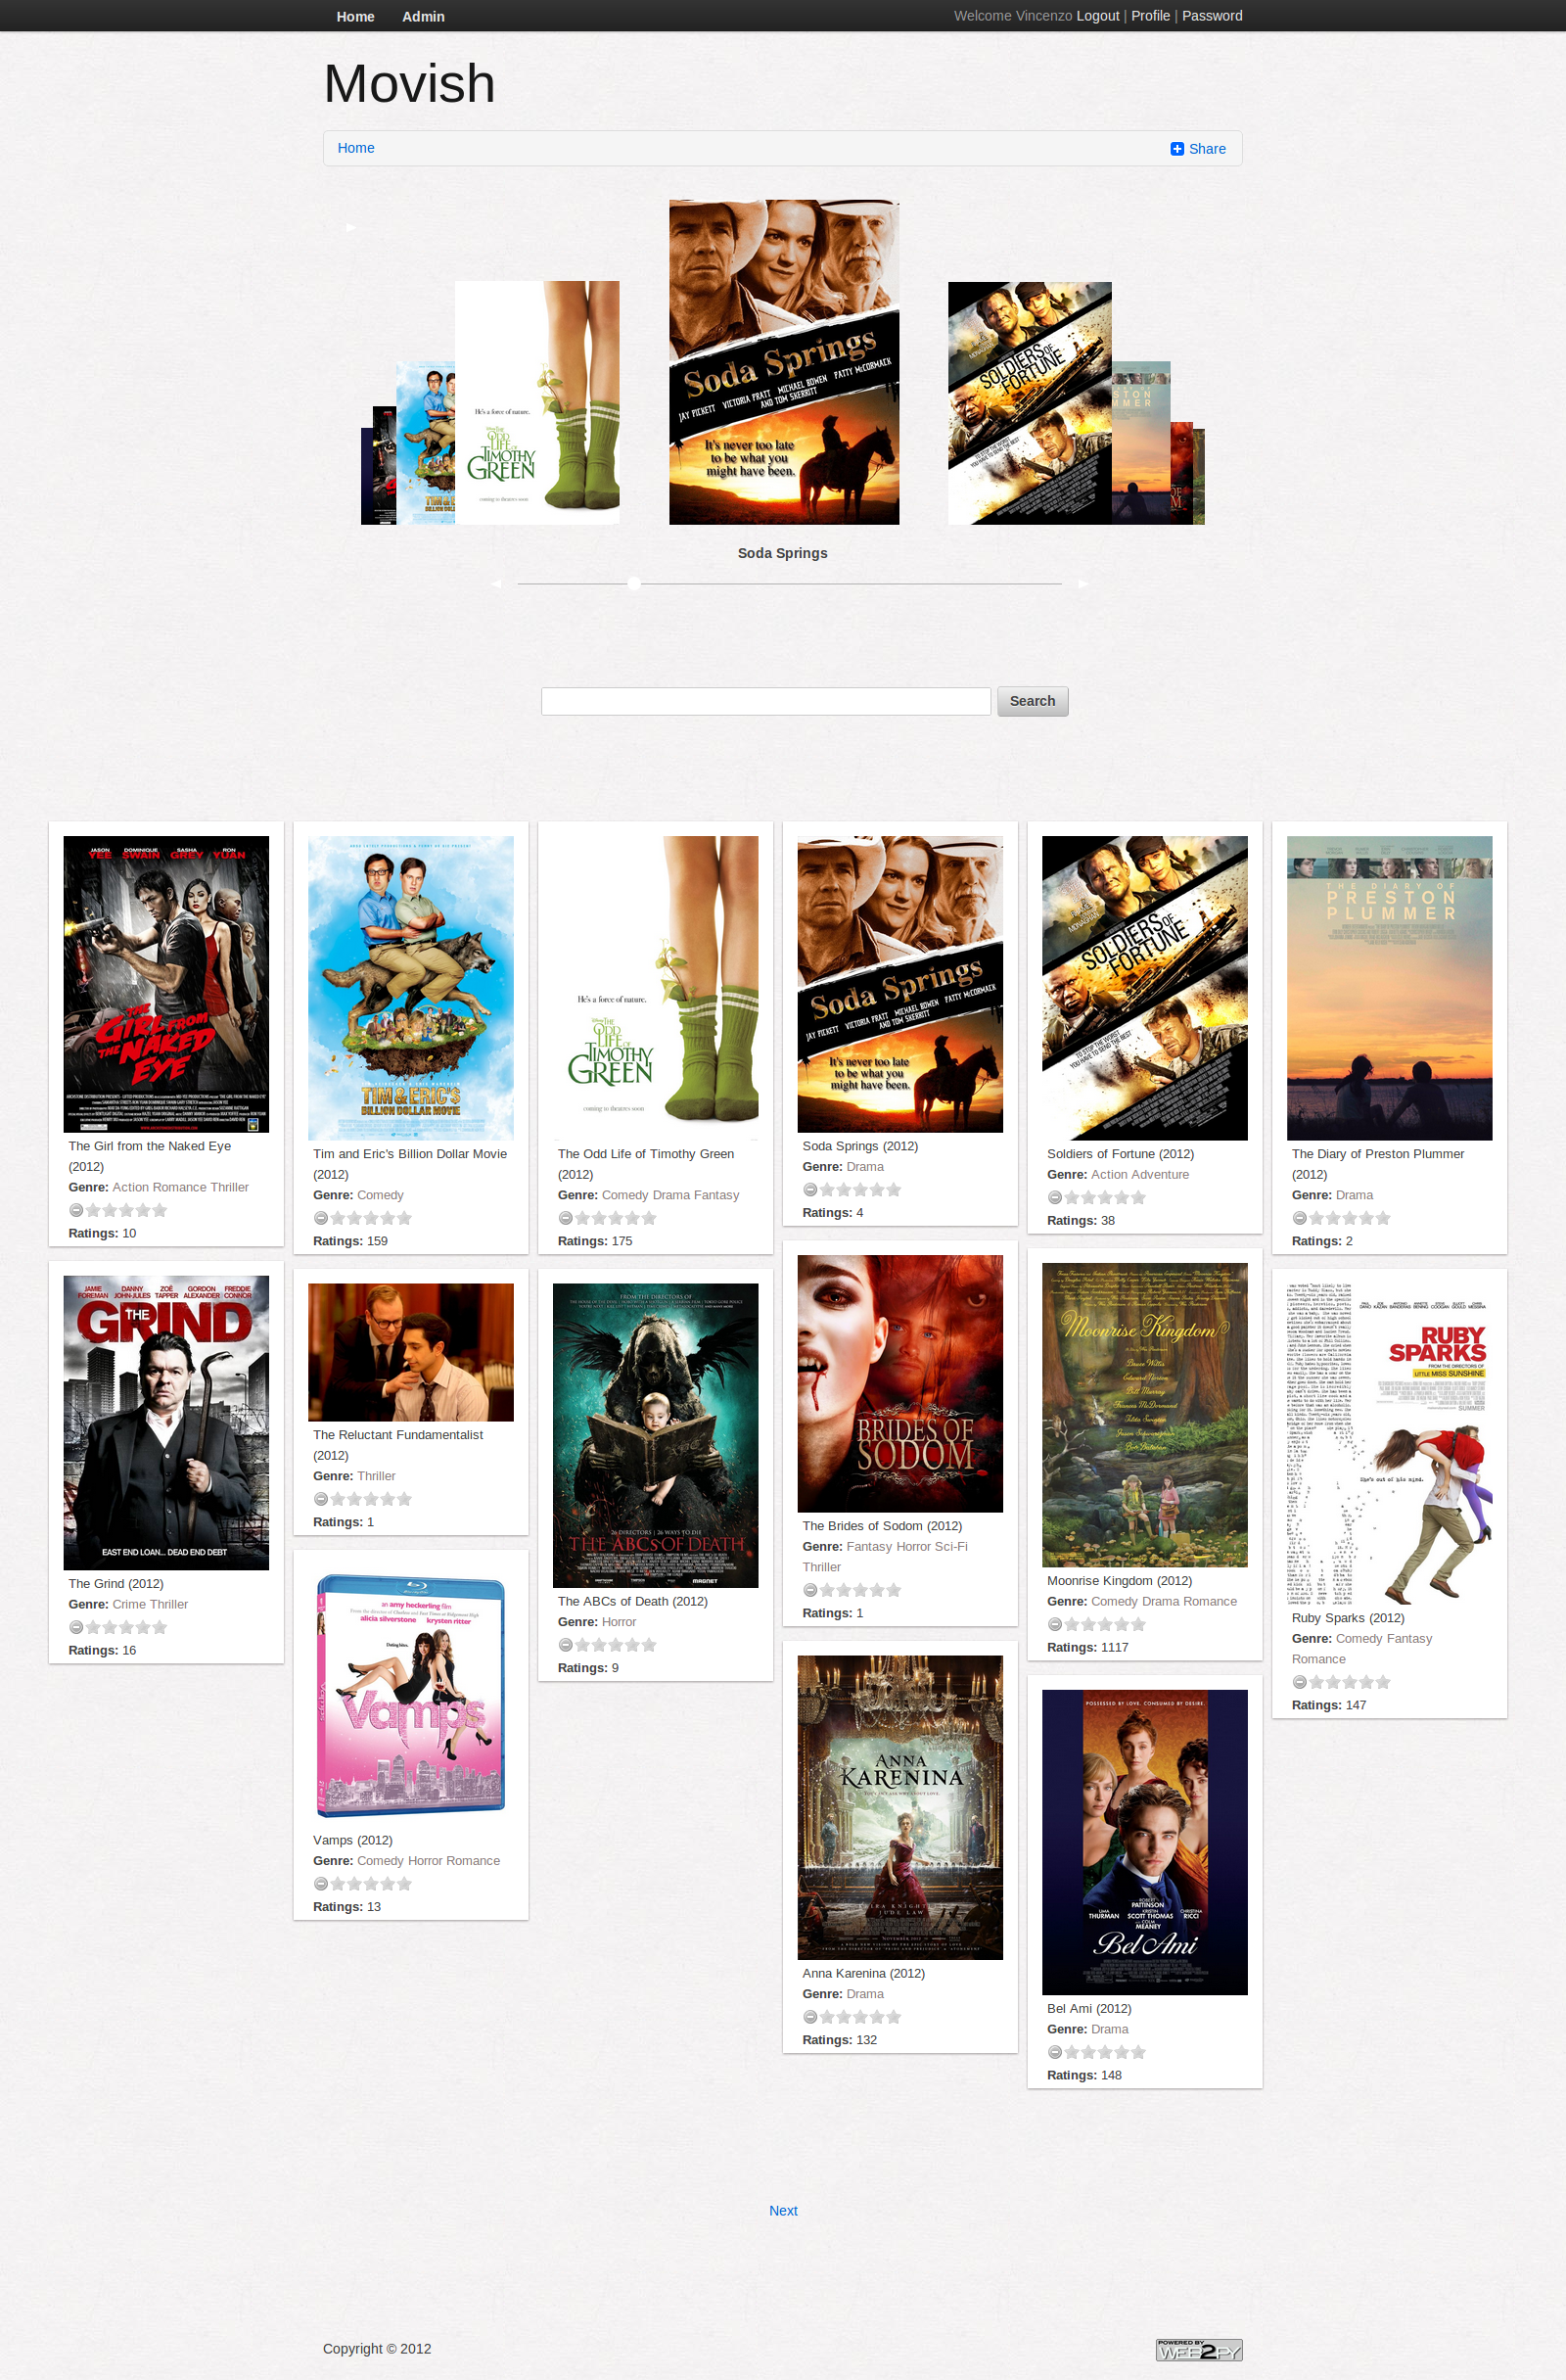
\includegraphics[width=\textwidth]{figures/movish-homepage.png}
  \caption{Movish homepage}
  \label{fig:movish_homepage}
\end{figure}

The user can then click on a single cover of a movie or a title to open a second page that displays the details about a movie like on figure \ref{fig:movie_detail}.

\begin{figure}
  \centering
  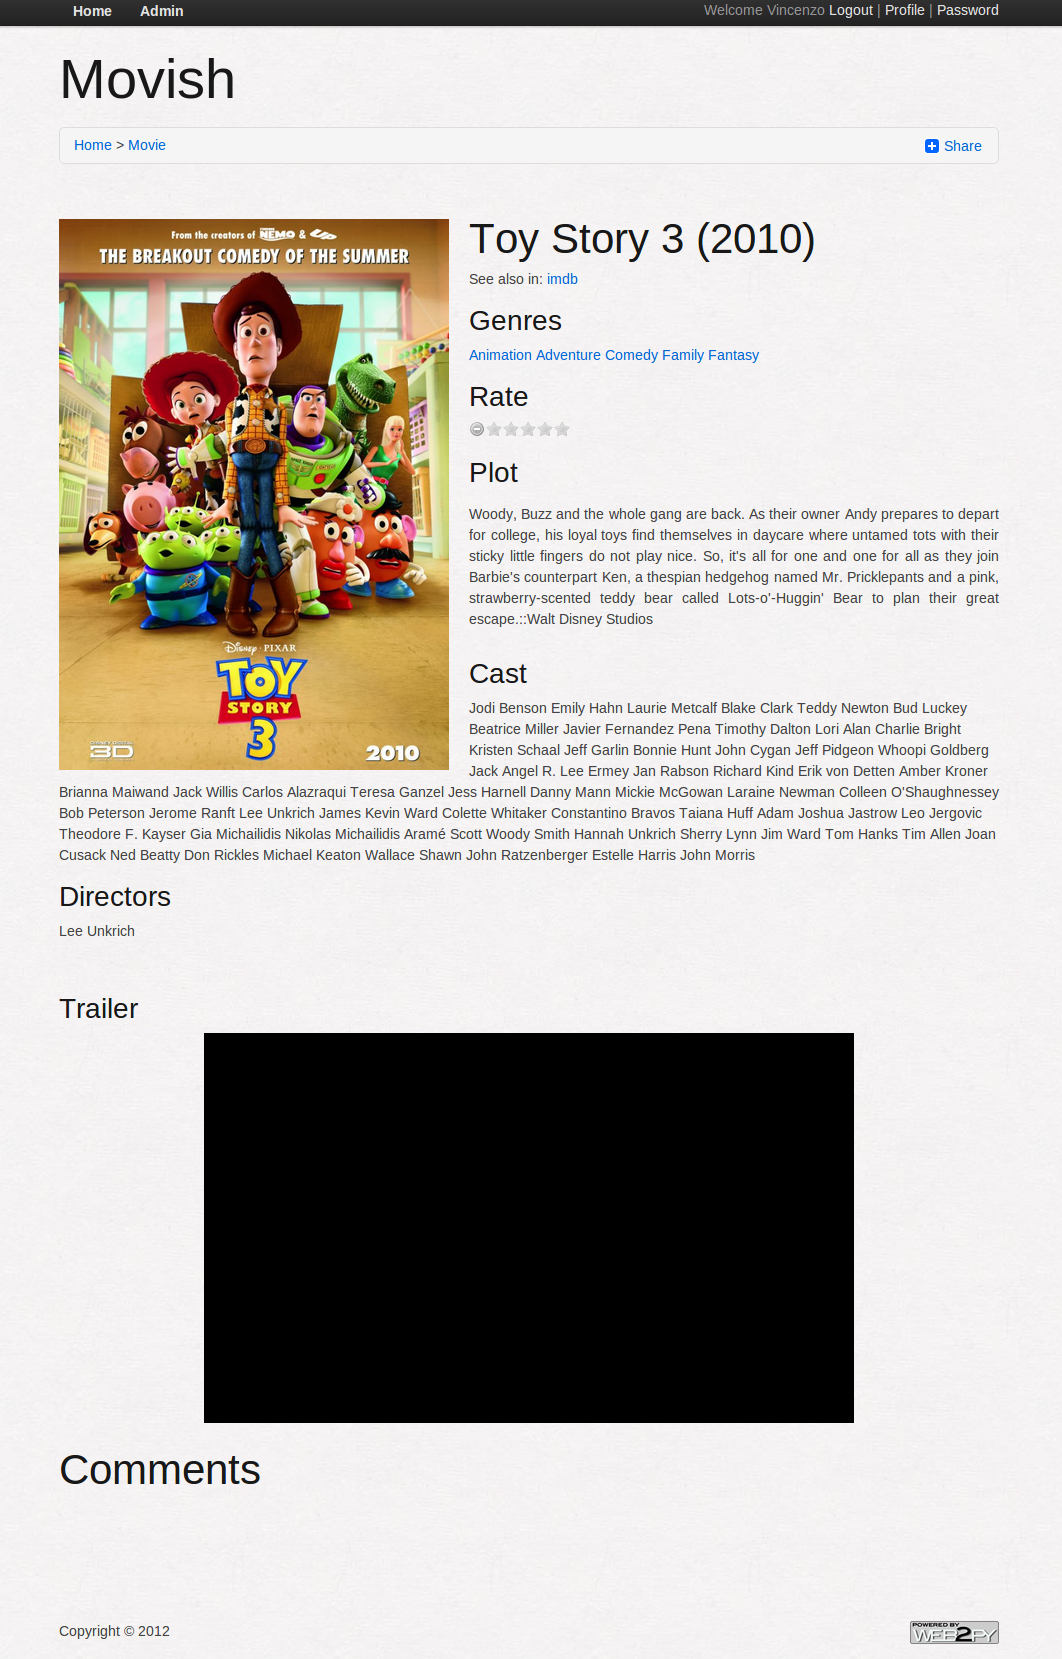
\includegraphics[width=\textwidth]{figures/movie-detail.png}
  \caption{Movie detail}
  \label{fig:movie_detail}
\end{figure}

The movie detail page will display the title, the imdb reference the genres, the plot, the members of the cast and the directors. On the side there is a big version of the movie cover that is used also in the listing of the catalog page. If there are comments of the users about the movie those are shown at the bottom of the page. If there is a trailer of the movie it will be also displayed but not played by default.

The detail page has been designed to be as clear and simple as possible displaying all the information about the movie in a single page. There is also a share button to share the link of a specific movie to a social network of your choice including Facebook, Twitter and Google plus.

\subsection{Admin interface}
\label{sec:admin_interface}


\begin{figure}
  \centering
  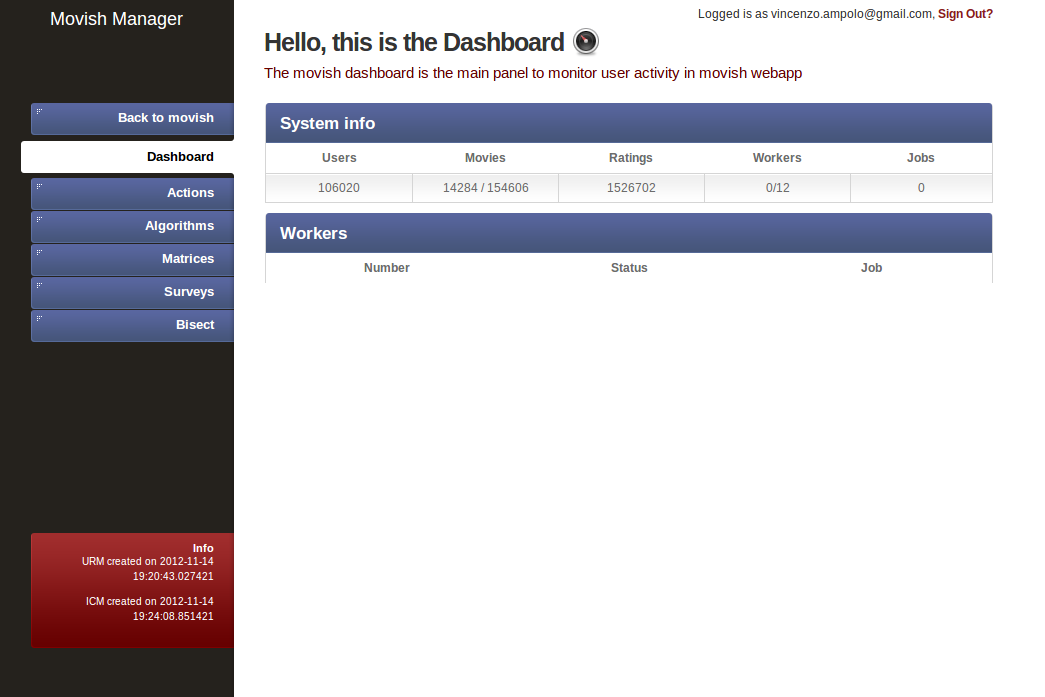
\includegraphics[width=\textwidth]{figures/admin_page.png}
  \caption{Movish admin mode homepage}
  \label{fig:admin_mode_homepage}
\end{figure}

The admin mode is shown in figure \ref{fig:admin_mode_homepage}. The admin has a different layout with a big menu on the left and a white space on the right in order to display information and content.
One of the main features of Movish is that the whole system can be managed by this admin interface.

The main page, or the dashboard, shows useful information of the status of the system. It displays the number of users in the system, the number of movies with full information, the number of movies that lack some information, the number of ratings in the system, the number of active and total workers and the number of pending tasks/jobs. In the dashboard there is also a table that is automatically generated with all the running worker and the task that they are working on. So the admin can see in which state is the system just loading a single page.

Every menu self expands as soon as the user clicks on it using a javascript function that enables a light animation.

\begin{figure}
  \centering
  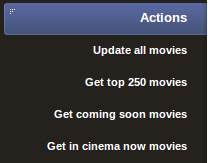
\includegraphics[width=0.4\textwidth]{figures/menu_actions.png}
  \caption{Actions menu}
  \label{fig:actions_menu}
\end{figure}

The actions menu in figure \ref{fig:actions_menu} shows all the possible actions that the admin can do to the system. The admin can launch an update all movies task, a get top 250 movies on imdb task, a get coming soon movies from imdb task or get in cinema now movies task. Each click will generate and Ajax \cite{ajax} call that will add the respective task to the scheduler. For each action the user receives a message saying that the operation has been added to the system. Each task will then be picked up by a worker selected by the scheduler and will execute it. The output of the task is directly written in the database and it is basically an insert or update operation on the database.

\begin{figure}
  \centering
  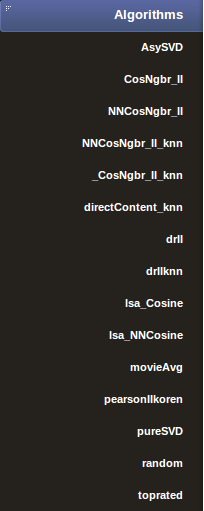
\includegraphics[width=0.4\textwidth]{figures/algorithms_menu.png}
  \caption{Algorithms menu}
  \label{fig:algorithms_menu}
\end{figure}

When the Algorithms menu in figure \ref{fig:algorithms_menu} is clicked, a list of all the algorithms located in the ``modules/algorithms'' sub-directory of the project is created and displayed. Each algorithm can be clicked. As soon as it is, the information about that specific algorithm is displayed. Figure \ref{fig:algorithms_menu} displays all the algorithms that are available in the system as for now. 
\begin{figure}
  \centering
  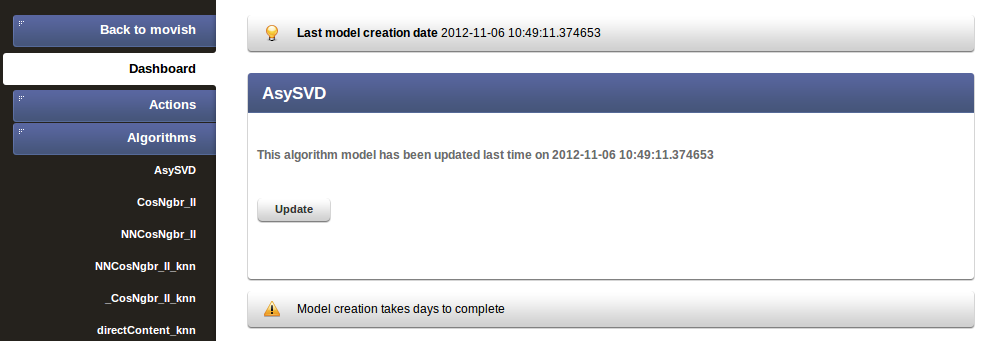
\includegraphics[width=\textwidth]{figures/algorithm_detail.png}
  \caption{Algorithm detail}
  \label{fig:algorithm_detail}
\end{figure}

Adding a new algorithms is easy: the administrator has to add all the relevant files about an algorithm to the \textit{modules/algorithms} directory. The system in fact has automatic discovering facilities to detect all the available algorithms. The algorithms should respect a common set of input and a common set of output. The reader can discover more about how to add an algorithm on section \ref{sec:structure}.

\begin{figure}
  \centering
  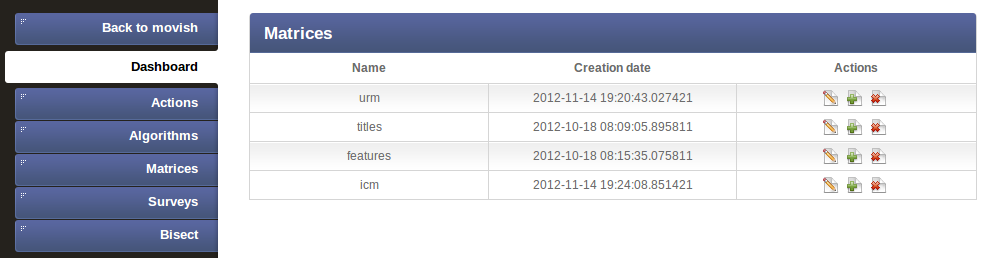
\includegraphics[width=\textwidth]{figures/matrices_detail.png}
  \caption{Matrices menu detail}
  \label{fig:matrice_menu}
\end{figure}

Figure \ref{fig:matrice_menu} shows the detail of the matrices in the system. It is displayed if the administrator clicks on the \textbf{Matrices} menu item. It shows the presence of the \ac{ICM}, \ac{URM}, titles an features vector. From the \textbf{action} column the user can select to download the matrice or vector, to schedule the creation of a new one or to delete it.

\begin{figure}
  \centering
  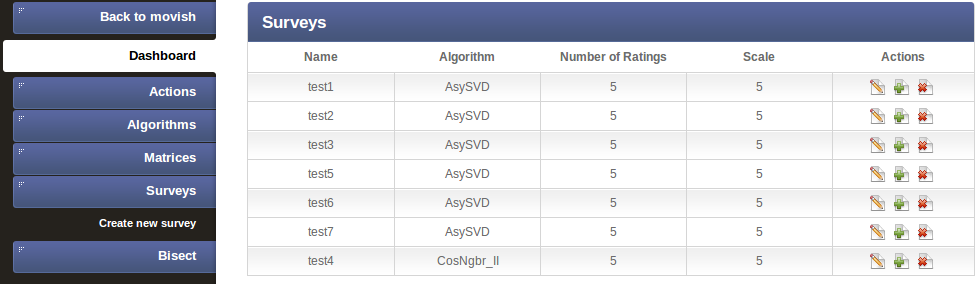
\includegraphics[width=\textwidth]{figures/survey_menu.png}
  \caption{Surveys menu}
  \label{fig:surveys_menu}
\end{figure}

Clicking on the \textbf{Surveys} button in the menu will open a sub menu for creating a new survey, called \textbf{Create new survey}, and will show all the surveys in the system. As for the \textbf{Matrices} menu, there is a \textit{Actions} column to download the data about the survey, to stop it from being available to the users or to delete it from the system. Clicking on \textbf{Create new survey} will cause the content portion of the page to load a form for submitting a new survey like on figure \ref{fig:create_survey}.

\begin{figure}
  \centering
  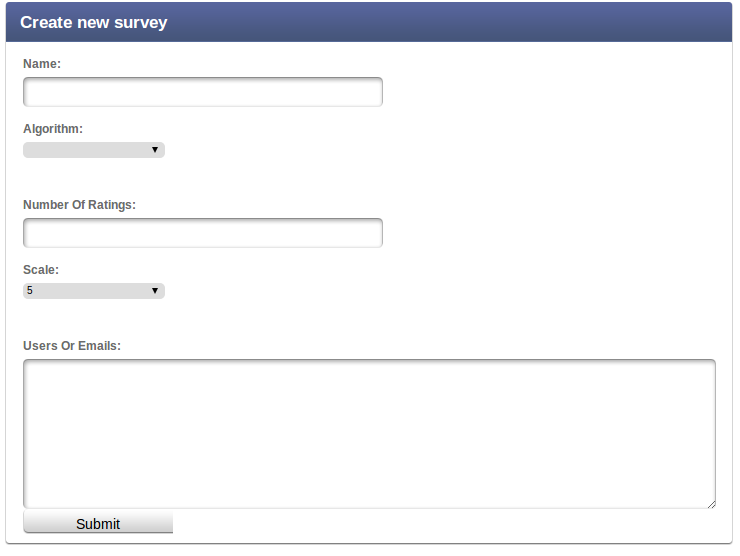
\includegraphics[width=\textwidth]{figures/create_survey.png}
  \caption{Create survey}
  \label{fig:create_survey}
\end{figure}

The administrator has to pick a name for the new survey, choose an algorithm from the drop down list which is, live for the \textbf{Algorithms menu} generated on the fly looking at the directory structure, the number of ratings that the user will perform

YOU HAVE TO CHANGE THIS

\begin{figure}
  \centering
  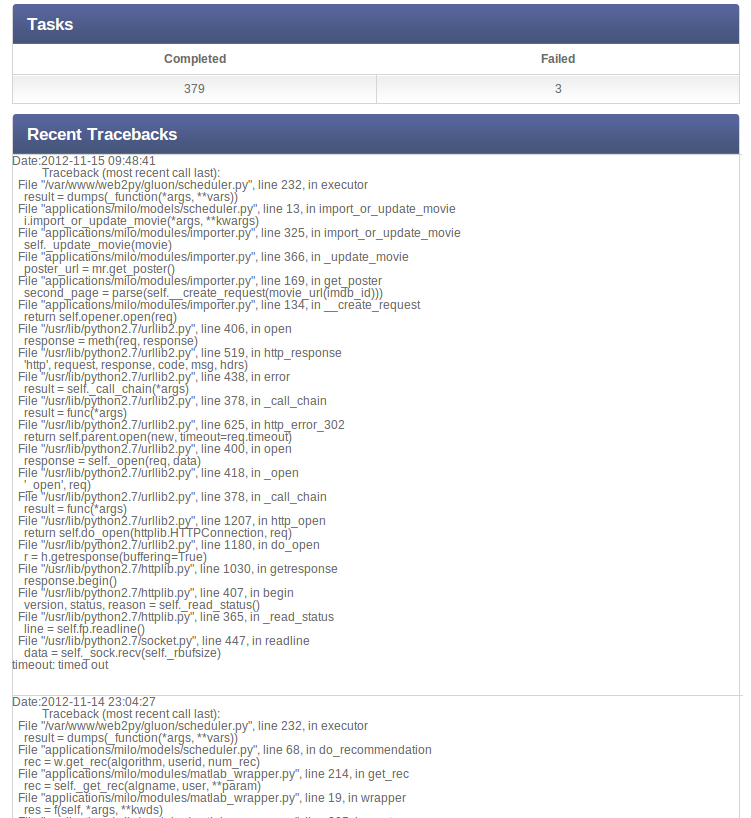
\includegraphics[width=\textwidth]{figures/bisect.png}
  \caption{Bisect menu}
  \label{fig:bisect_menu}
\end{figure}

Figure \ref{fig:bisect_menu} shows the last menu item, \textbf{Bisect}. This is for meant for debbugging purposes. In Bisect the administrator can see the total complete tasks and the failed ones. For the last ten failed tasks there is a detailed traceback with useful information about the error and hopefully in how to fix it. In the figure there is a problem with a timed out connection for example. Of course the \textbf{Bisect} section is not meant to do be a full debugger but it may be really helpful to discover bad uses of the software without even opening an code editor.

\subsection{Scheduler}
\label{sec:scheduler}

The scheduler is a fundamental part of the system. It is embedded in the web2py \cite{web2py} framework and is formed by workers that implement a distributed way to assign task to each worker and solve it. It is perfectly integrated with the underlying database which allows easy monitoring and modifying like exposed in section \ref{sec:admin_interface} in the admin dashboard.

\begin{figure}
  \centering
  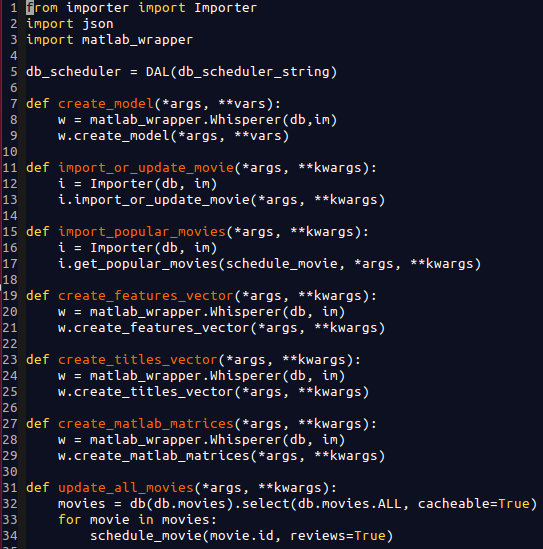
\includegraphics[width=\textwidth]{figures/scheduler1.png}
  \caption{Scheduler 1/2}
  \label{fig:scheduler1}
\end{figure}

\begin{figure}
  \centering
  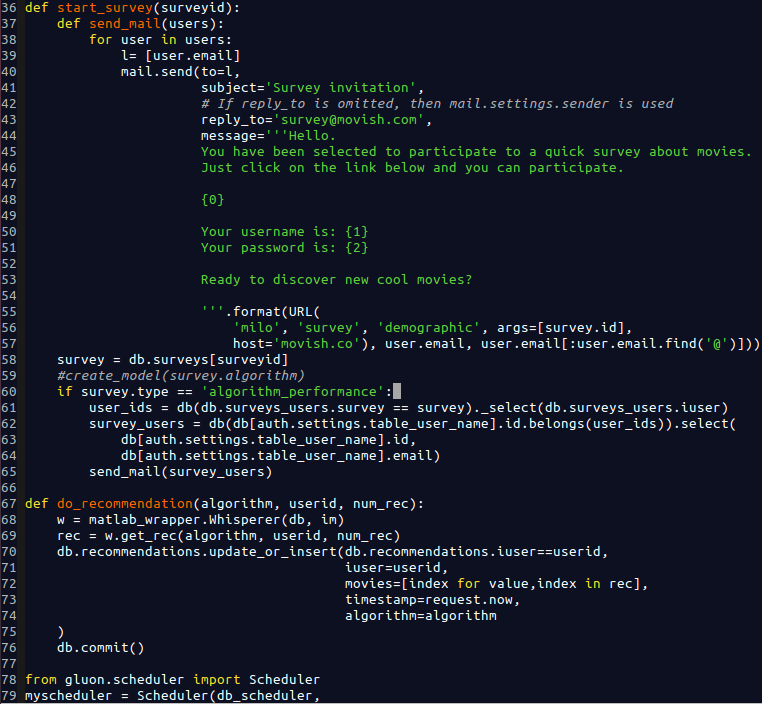
\includegraphics[width=\textwidth]{figures/scheduler2.png}
  \caption{Scheduler 2/2}
  \label{fig:scheduler2}
\end{figure}

The scheduler is mainly configured in file \textit{models/scheduler.py} which is shown in Figure \ref{fig:scheduler1} and Figure \ref{fig:scheduler2}. It mainly imports the importer module of which we will talk in section \ref{sec:importer} and encapsulates the most important functions in scheduler tasks.
The defined functions are:
\begin{itemize}
\item \textbf{create\_model}. This function takes a name of an algorithm as its input and creates a model for the given algorithm. If the URM and the ICM are not in the system, they are created too.
\item \textbf{import\_or\_update\_movie}. This is one of the most important scheduler tasks. It gets scheduled as soon as a movie with no title, no cover or no year information is displayed to the user. It fetches the information about a movie from imdb, surfs between all the reviews and collects them, also includes all the imdb users that gave a review to the movish system. It thus queries youtube in order to find a trailer for the movie and it if finds it, updates the movie info. Given all the operations that this function is capable of it resembles the core part of the auto updating feature of the system.
\item \textbf{import\_popular\_movies}. This function surf the imdb popular movies page and add schedules all the movies in that page for an update thanks to \textit{import\_popular\_movies}.
\item \textbf{create\_features\_vector}. This function simply creates the feature vector. It's is scheduled from the admin mode under the action menu as described in section \ref{sec:admin_interface}.
\item \textbf{create\_title\_vectors}. Like the previous function, this creates the titles vector and it's scheduled from the admin mode.
\item \textbf{create\_matlab\_matrices}. This task creates the \ac{URM} and \ac{ICM} to be used for the model creation.
\item \textbf{update\_all\_movies}. Using \textit{import\_or\_update\_movie} this task cycles in all the movies in the system and schedule them for a update.
\item \textbf{start\_survey}. When a survey is added to the system this function is responsible of setting up the survey and send a mail to each user that has been indicated to perform the survey to let them know that the survey is ready.
\item \textbf{do\_recommendation}. Given an algorithm, a userid and a integer N, this task stores on database a recommendation for the given algorithm of N movies. This function is the core function for the recommendation engine. It has been performed as a task because it can take more than 40 seconds in the given hardware which is a Xenon quad core at 3Ghz with 16gb of ram. 40 seconds are not feasible for a web application that has to be as fast as it can. Thus this task has been added.
\end{itemize}

\subsection{Importer}
\label{sec:importer}

The importer is the part of the system that implements all the automatism and makes the system able to auto update with new movies. The importer is defined in file \textit{modules/importer.py}. This file defines a \textbf{Importer} and \textbf{MediaRetriever} class. The MediaRetriever class is able to perform parsing from pages of imdb.com and youtube.com that are fetched by the crawler of section \ref{sec:crawler}. The Importer class uses the MediaRetriever to get the trailer and the cover for a movie, it also uses the imdbpy \cite{imdbpy} library to retrieve information about the movie and store into database. The Importer is capable to parse all the imdb.com reviews, to generate metadata for each movie and add them to database.

\begin{figure}
  \centering
  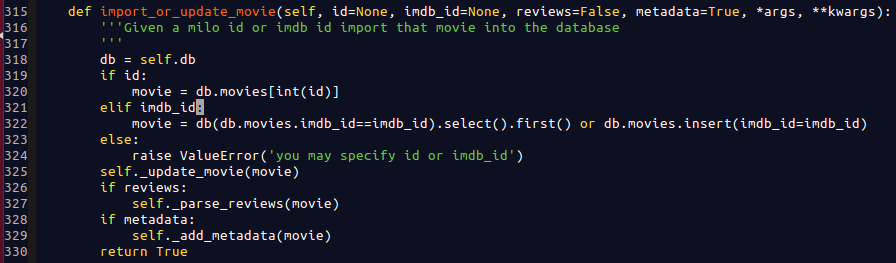
\includegraphics[width=\textwidth]{figures/importer_core_function.png}
  \caption{Importer core function}
  \label{fig:importer_core}
\end{figure}

The core function of the importer is shown in Figure \ref{fig:importer_core}. It is basically the code called by the \textbf{import\_or\_update\_movie} of the scheduler exposed in secion \ref{sec:scheduler}.

The importer connects to the crawler via a proxy service installed in the same server at port 8118. The crawler talks with the importer via a trasparent http proxy such that the crawler can be disabled at any time without affecting the overall system.

\subsection{Crawler}
\label{sec:crawler}

As soon as the system started getting information from both youtube and imdb the incoming traffic to these application have been throttled. In order to be able to access those sources a Tor based proxy has been set up.

Tor \cite{tor} is a network of virtual tunnels that allows people and groups to improve their privacy and security on the Internet. It also enables software developers to create new communication tools with built-in privacy features. Tor provides the foundation for a range of applications that allow organizations and individuals to share information over public networks without compromising their privacy.

In movish, tor represent the crawler thanks to whom the importer can communicate to imdb.com and youtube.com in an anonymous way using different ip addresses every 10 minute in order to overcome to the bandwidth limitation that those two website impose to their users. Without this proxy the required time to create a useful dataset would require almost a year.

\begin{figure}
  \centering
  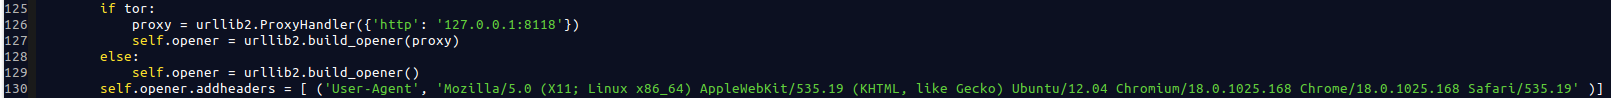
\includegraphics[width=\textwidth]{figures/crawler_setting_code.png}
  \caption{Importer setting the crawler as a gateway code}
  \label{fig:importer_setting_crawler}
\end{figure}

Figure \ref{fig:importer_setting_crawler} shows a small snippet of code from the \textbf{Importer} that sets up the \textbf{Crawler} as a proxy to reach both youtube and imdb. The code exposed is located at file named \textit{modules/importer.py} at line 125. Thanks to the urllib2 python library flexibility it is possible to configure each request to use a proxy creating an \textit{opener} object. Last line adds an user agent signature to each request to act like a real user opening the requested page.

\subsection{Recommendation engine}
\label{sec:recommendation_engine}

The recommendation engine is the section of the application responsible of making and retrieve recommendations using a Matlab \cite{matlab} engine. It was one of the constraints of the system since Milo because all the algorithms developed by the research group at Politecnico di Milano are implemented using that program. Matlab is heavily used in many courses at Politecnico di Milano and many other universities around the world, the Netflix competition \cite{netflixprize} was also released using Matlab .mat files.

There is one single file in which matlab is imported and used in the entire system and it is in the \textit{modules/matlab\_wrapper.py}. The file contains mainly a object called \textbf{Whisperer}. This object exports all the function to create the matlab matrices \ac{ICM} and \ac{URM}, the titles and features vectors, the model for each supported algorithm and the recommendation for a given user. The object is also able to talk with the database in order to retrieve the correct data.

\begin{figure}
  \centering
  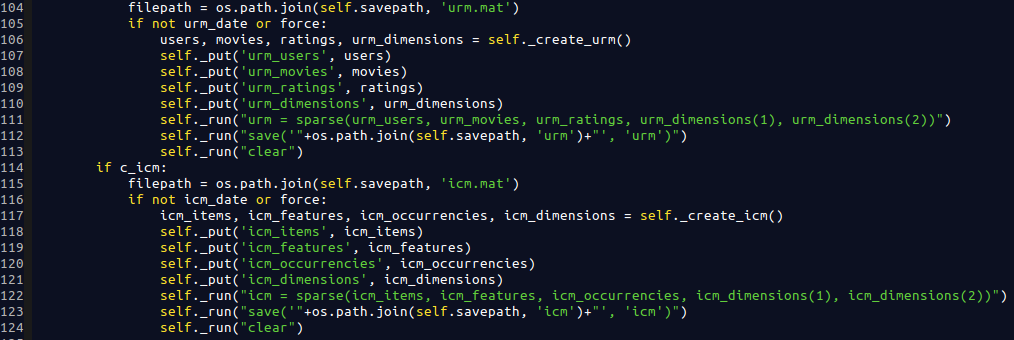
\includegraphics[width=\textwidth]{figures/urm_and_icm_creation.png}
  \caption{URM and ICM creation}
  \label{fig:urm_and_icm_cration}
\end{figure}

Figure \ref{fig:urm_and_icm_cration} shows a snippet used for the \ac{URM} and \ac{ICM} generation. The variables are inserted in the matlab environment thanks to the \textit{self.\_put()} function while the matlab commands are run thanks to the \textit{self.\_run()} function. One of the big improvements of this piece of the application compared to Milo is the optimization performed at memory level by replacing matrices with sparse matrices. This change imposed a change in the whole way the matrices are managed but it was able to drop memory requirements from 80Gb to 3Gb of \ac{RAM}. After the matrices are computed they are stored in Matlab .mat files for easy retrieval from the admin interface exposed in section \ref{sec:admin_interface}.

Each function that deals with matlab uses a \textbf{@matlab} python decorator. A decorator in python is a function that is applied to other functions. In this case the @matlab decorator ensures that the function that will be called using matlab will find a clear environment from other variables. This enhancement prevent the system from keep loading and unloading matlab environments for each function to call. The system keeps a single matlab session ready for each function, each function that is called cleans the environment after it exits thanks to the decorator instead.

\begin{figure}
  \centering
  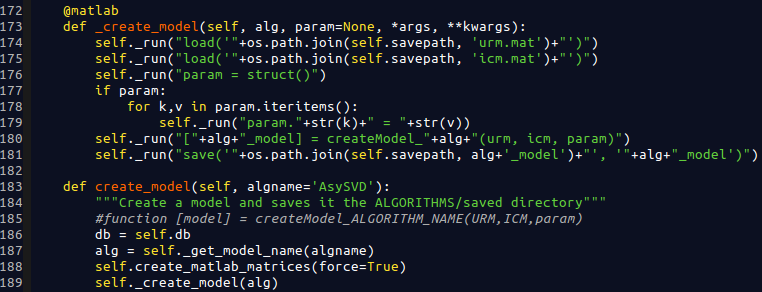
\includegraphics[width=\textwidth]{figures/create_model.png}
  \caption{Create model code}
  \label{fig:create_model}
\end{figure}

Figure \ref{fig:create_model} shows the code to create a model. As you can see the action is performed by two functions. The first one called \textbf{create\_model} ensures that the \ac{URM} and the \ac{ICM} are created. It thus calls the \textbf{\_create\_model} function that manages a matlab session, this is why it has the \textbf{@matlab} decorator, and performs the actual recommendation calling the right function name for the given algorithm in order to create the model.

The recommendation is done in a similar way of the model creation from the \textbf{get\_rec} function. It accepts three parameters being the algorithm name and the user id. It then retrieve the user profile and performs the recommendation for the given algorithm if a model exists.

\begin{figure}
  \centering
  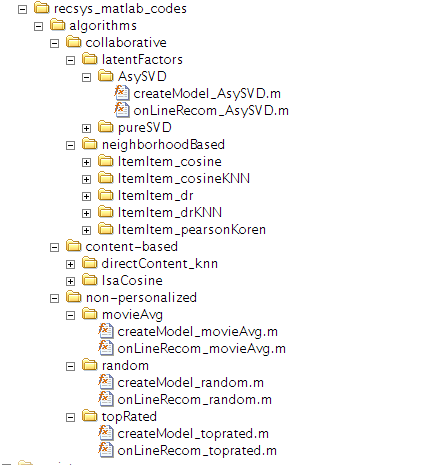
\includegraphics[width=\textwidth]{figures/matlab_algorithms_tree.png}
  \caption{Matlab algorithm tree structure}
  \label{fig:matlab_tree_structure}
\end{figure}

The recommendation engine has also an auto discovery functionality of new algorithms. When generating the lists of algorithms it simply looks in the \textit{modules/algorithms/recsys\_matlab\_codes/algorithms/} directory and look for files which name that starts with \textbf{onLineRecom}. In fact all the algorithm have the form of \textit{onLineRecom\_algorithm.m}. For each algorithm found, the relative model creation function is looked up searching in the same directory of the algorithm for a \textit{createModel\_algorithm.m}. That file contains the function to generate the model for a given algorithm. Figure \ref{fig:matlab_tree_structure} shows the matlab algorithms tree structure. Each algorithm is categorized to be collaborative, content based or non personalized. For each class of algorithms, there are all the relevant sub classes.

All the computations that result in a creation of a file for matlab store the newly created file in the \textit{modules/elaborated\_models/}.

\section{Structure}
\label{sec:structure}

The project structure is based on web2py \cite{web2py} one. The project has been published on GitHub \cite{github}. GitHub defines itself like ``the best place to share code with friends, co-workers, classmates, and complete strangers. Over two million people use GitHub to build amazing things together''. GitHub is a webapp designed to share code using the git \cite{git-scm} revision control system. The application is composed mainly by the controllers, views, static, modules and models directory. All the other directories are the basic template of a web2y application.

\begin{itemize}
\item \textbf{controllers} directory contains all the controllers of the application. \textit{admin.py} defines the controllers of the admin interface \ref{sec:admin_interface} with all the functions and the actions that the administrator can perform. \textit{default.py} is the default controller which is called when the homepage is called. it has the \textit{index} function that perform the basic visualization of the list of movies. \textit{movie.py} is the controller for displaying the details of a movie. \textit{rating.py} is the controller that takes care of performing ratings for a movie. This last controller is different from the other since it is designed to works as a module for other controllers. In fact the rating of a movie is always associate with a movie, so this controller is responsible of generating the correct stars indicating the rating and load the previous rating for a movie if the user already gave a rating for that movie. \textit{survey.py} is the controller that handles all the survey creation.
\item \textbf{models} directory contains all the data structures used in the application. The \textit{db.py} defines all the database structure the reader can have a look to the ER diagram on section \ref{sec:movish}. \textit{menu.py} defines the context menu that is displayed to the user. It is the menu on top on the black line which never changes and is the landmark for the user. \textit{scheduler.py} this file defines the scheduler tasks. It uses the web2py automatic task discovering features to add the functions to the scheduler. We analyzed the code of the scheduler on secion \ref{sec:scheduler}. \textit{whisperer.py} contains all the function that are called by the application to schedule tasks of the scheduler. Thanks to this file adding a task to the scheduler is easy like calling a function.
\item \textit{modules} directory contains all the matlab algorithm under the  \textit{algorithms} directory and all the models under \textit{elaborated\_models}. The \textit{countries.py} file defines the list of all countries in the world used by the surveys while asking the demographic data. \textit{importer.py} defines the Importer we talked in section \ref{sec:importer}. \textit{matlab\_wrapper.py} is the only file that interact with the matlab engine, thus is the only file that imports pymatlab \cite{pymatlab}. \textit{metadata.py} is the file used to set up the python \ac{nltk} \cite{nltk}. Nltk is a leading platform for building Python programs to work with human language data. It provides easy-to-use interfaces to over 50 corpora and lexical resources such as WordNet, along with a suite of text processing libraries for classification, tokenization, stemming, tagging, parsing, and semantic reasoning. Nltk is used by Movish to perform plot tagging and extract the metadata for the movie. These metadata are useful for the \ac{ICM} generation as explained in section \ref{sec:Input}.
\item \textit{static} directory contains all the static content of the application. Mainly all the css the the images.
\item \textbf{views} directory contains all the html files that are used for outputting the data generated by the controllers to the user.
\end{itemize}

\section{Dataset}
\label{sec:dataset}

The initial dataset used for milo was the one used for the netflix competition \cite{netflixprize} but since it was released in 2001 it was soon figured out that it was pretty outdated and not useful for real recommendations with users. This is why in milo there were a basic importer to get the informations from the imdb.com website. That importer was only able to retrieve basic information. In movish the importer is now able to parse imdb.com directly, to talk to imdb thanks to the imdbpy \cite{imdbpy} library and to parse youtube pages directly. It is also able to parse all reviews in different pages of a movie and get the ratings.

Having this powerful importer, during three continuous months of scraping the imdb.com website, the majority of movies from the 1950 until now have been imported in the system. Resulting in 154606 distinc titles and 106266 distinct users as for Nov 23th 2012. In order to keep the datased up to date, the admin can create a task of updating all the movies via the admin interface explained in secion \ref{sec:admin_interface}. The system is also able to automatically detect if a movie has not all the information and schedules a task for updating the movie information as explained in figure \ref{fig:movie_update}.

\begin{figure}
  \centering
  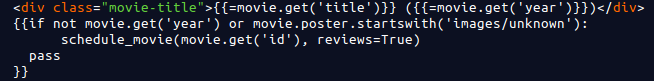
\includegraphics[width=\textwidth]{figures/auto_update_movie.png}
  \caption{Automatically schedule a movie information update}
  \label{fig:movie_update}
\end{figure}

When the movie is displayed if the year field is missing or if the poster of the movie is not defined, the movies is then scheduled for an update. The system also provide a cronjob to automatically fetch new reviews and new movies that are going to be released in the next five years or that have been released in the past five years. This ensures that the system has up to date movies an reviews from imdb distributing the load of updating the dataset during time.

This is one of the biggest improvement from ContentWise \cite{ContentWise} and enables new scenario and integration with other realtime or up to date system such as Facebook and Twitter.

\section{Conclusions}
\label{sec:movish_system_conclusions}

Movish is an extensible fully automatic recommendation survey system for movies. Thanks to its fundamental in bleeding edge technologies and functionalities it is able of self updating the dataset, perform async recommendations, and having a good look and feel thanks to the simple interface. It's architecture is composed by many independent pieces that collaborates each other as explained in section \ref{sec:architecture} minimizing the point of failures that were one of the main problems in Milo. 

There are some factor that may limit the evolution of Movish in the long term:

\begin{itemize}
\item \textbf{Matlab dependence}. Having a matlab engine to support existing algorithms was a goal of the project but matlab has been proved, during the movish implementation, that it is not suitable for real time recommendation systems since it requires too many resources and it is too slow compared to native python implementation. In fact if the recommendation algorithms were implemented in python the system would require much less resources and be much faster than it is now. So in the future developing an alternate recommendation engine, maybe in python, would be very helpful and would not impact with the overall system.
\item \textbf{Improved security}. As for now all the communication with the server is performed via insecure http connections. Switching to https would protect user data transferred over the internet and block password hijacking attempts.
\item \textbf{Improve sources}. As for now only imdb.com and youtube.com are used as sources. Even if they are the most comprehensive sources available there are many more sources with ratings online that could be imported in the system to perform better recommendations.
\end{itemize}

In this chapter we didn't talk about survey management. Since it is another big feature of the web application, chapter \ref{chapter:<survey_management>} will explain how Movish handles surveys, how to create one and how to add a new type of survey.

\acresetall